
\documentclass[../report.tex]{subfiles}
\begin{document}

\graphicspath{{img/}{../img/}}

\subsection{Business Logic Layer Design}

This section will regard implementation of the Business Logic Layer. The design objectives is for the layer to be transparent, supportable, reliable and testable. The rest of the chapter will discus how this was achieved in the implementation. 

%% <--- HEAD
\paragraph{Transparency}
In order to gain transparency in the BLL, Business Logic Layer, an Abstract Factory pattern with a regular Factory pattern on top has been used (see figure \ref{BLLclassdiagram}). This makes it possible to gain access to the concrete implementations of the Abstract Factory from the Service Layer while only exposing one concrete class, namely the BusinessLogicEntryFactory. The design abstracts interface from concret implementation and enables the Service Layer using the BLL to only depend on the interface and the factory, but not the concret implementations.

%% -----

%This makes the Business Logic Layer reasonably transparent. We could have gone for a very transparent design with a Facade pattern for instance. This would mean exposing one concrete class like we do now, but not exposing any interfaces. The way to access the Business Logic Layer would then be by calling a method in the facade class which then delegates the work to other classes in the Business Logic Layer. This would involve having a method in the facade class for each method in our entire Business Logic Layer making it enormously bloated which works against some of the other goals we are trying to achieve. So we went with the Entry Factory solution because it gives us some of the properties of a Facade Pattern without making a hugely bloated class.

%% --->

%% <--- HEAD

\paragraph{Supportability} The Abstract Factory also achieves supportability.
The subsystem is designed to easily support adding new logic
implementations. Adding new factories is not supported in the structure as the
developer would have to change the BusinessLogicEntityFactory. The advantage
of being able to do so is if different kind of logics supporting different
kind of persistence was needed. This is not needed in ShareIT, as the
persistence module is dependency injected (allowing persistence to be switched
by injecting other persistence implementation), and therefore this structure
suffices for the desired level of supportability.

% ------

%The Abstract Factory also helps with the supportability of our Business Logic Layer. The nature of an Abstract Factory makes it very easy to add support for new things by just adding a new factory. In our case the Entry Factory would also have to be updated with a method for creating the new type of factory. Adding completely new functionality is a bit more difficult since the Abstract Factory and/or the Abstract Products interface have to be changed. 

% ---> 

%%% This is not relevant to implementation... %%%
%The type of Abstract Factory we have implemented is a very standard kind. We went for this because it is a very reliable kind of Abstract factory compared to a more flexible version which uses parameters in the operations that create objects\footnote{http://www.silversoft.net/docs/dp/hires/pat3afso.htm}. That way of making an Abstract Factory is much less reliable since there is no type security for the products produced by the factories. This can be a big problem for the one who has to use the Abstract Factory.

% <--- HEAD

\paragraph{Reliability}
Reliability is achieved by having a standard factory on top (EntryFactory). This structure limits the BLL to only having one entry point and therefore being in better control of calls to the subsystem thereby removing the possibility of unsafe operations due to incorrect precedence. 

% ------

%Another thing that adds to the reliability of our BLL is the Entry Factory. Since it is the only concrete class we expose, all interaction with the BLL is limited to the methods that our Entry Factory contains. This makes it more difficult to perform unsafe operations.

% --->

% <--- HEAD

\paragraph{Testability}
As per the project test strategy every subsystem should be unit and integration tested. Therefore the subsystem is designed to be highly testable through interfacing.

The subsystem also included a test stub. The test stub facilitated ArtShare and SMU clients to be coded up against the logic before it was done. This facilitated parallel development in the project.

%\todo{Hvorfor hjælper interfaces på testability?}

% ------

%A lot of reliability also comes from testing so we made sure that our BLL is highly testable by interfacing almost everything so it can be unit tested effectively. Apart from interfacing the factories and the products as the Abstract Factory pattern specifies we also interfaced our MediaItemMapper so it could be tested separately. 

%Apart from testability the large amount of interfaces also made it possible for us to quickly make a test factory with a stub implementation. This allowed us to deploy something that the SMU students could work with very quickly while simultaneously working on the actual implementation. When the time came to deploy some of the actual implementation we just had to change factories.

% --->

\begin{figure}
\centering
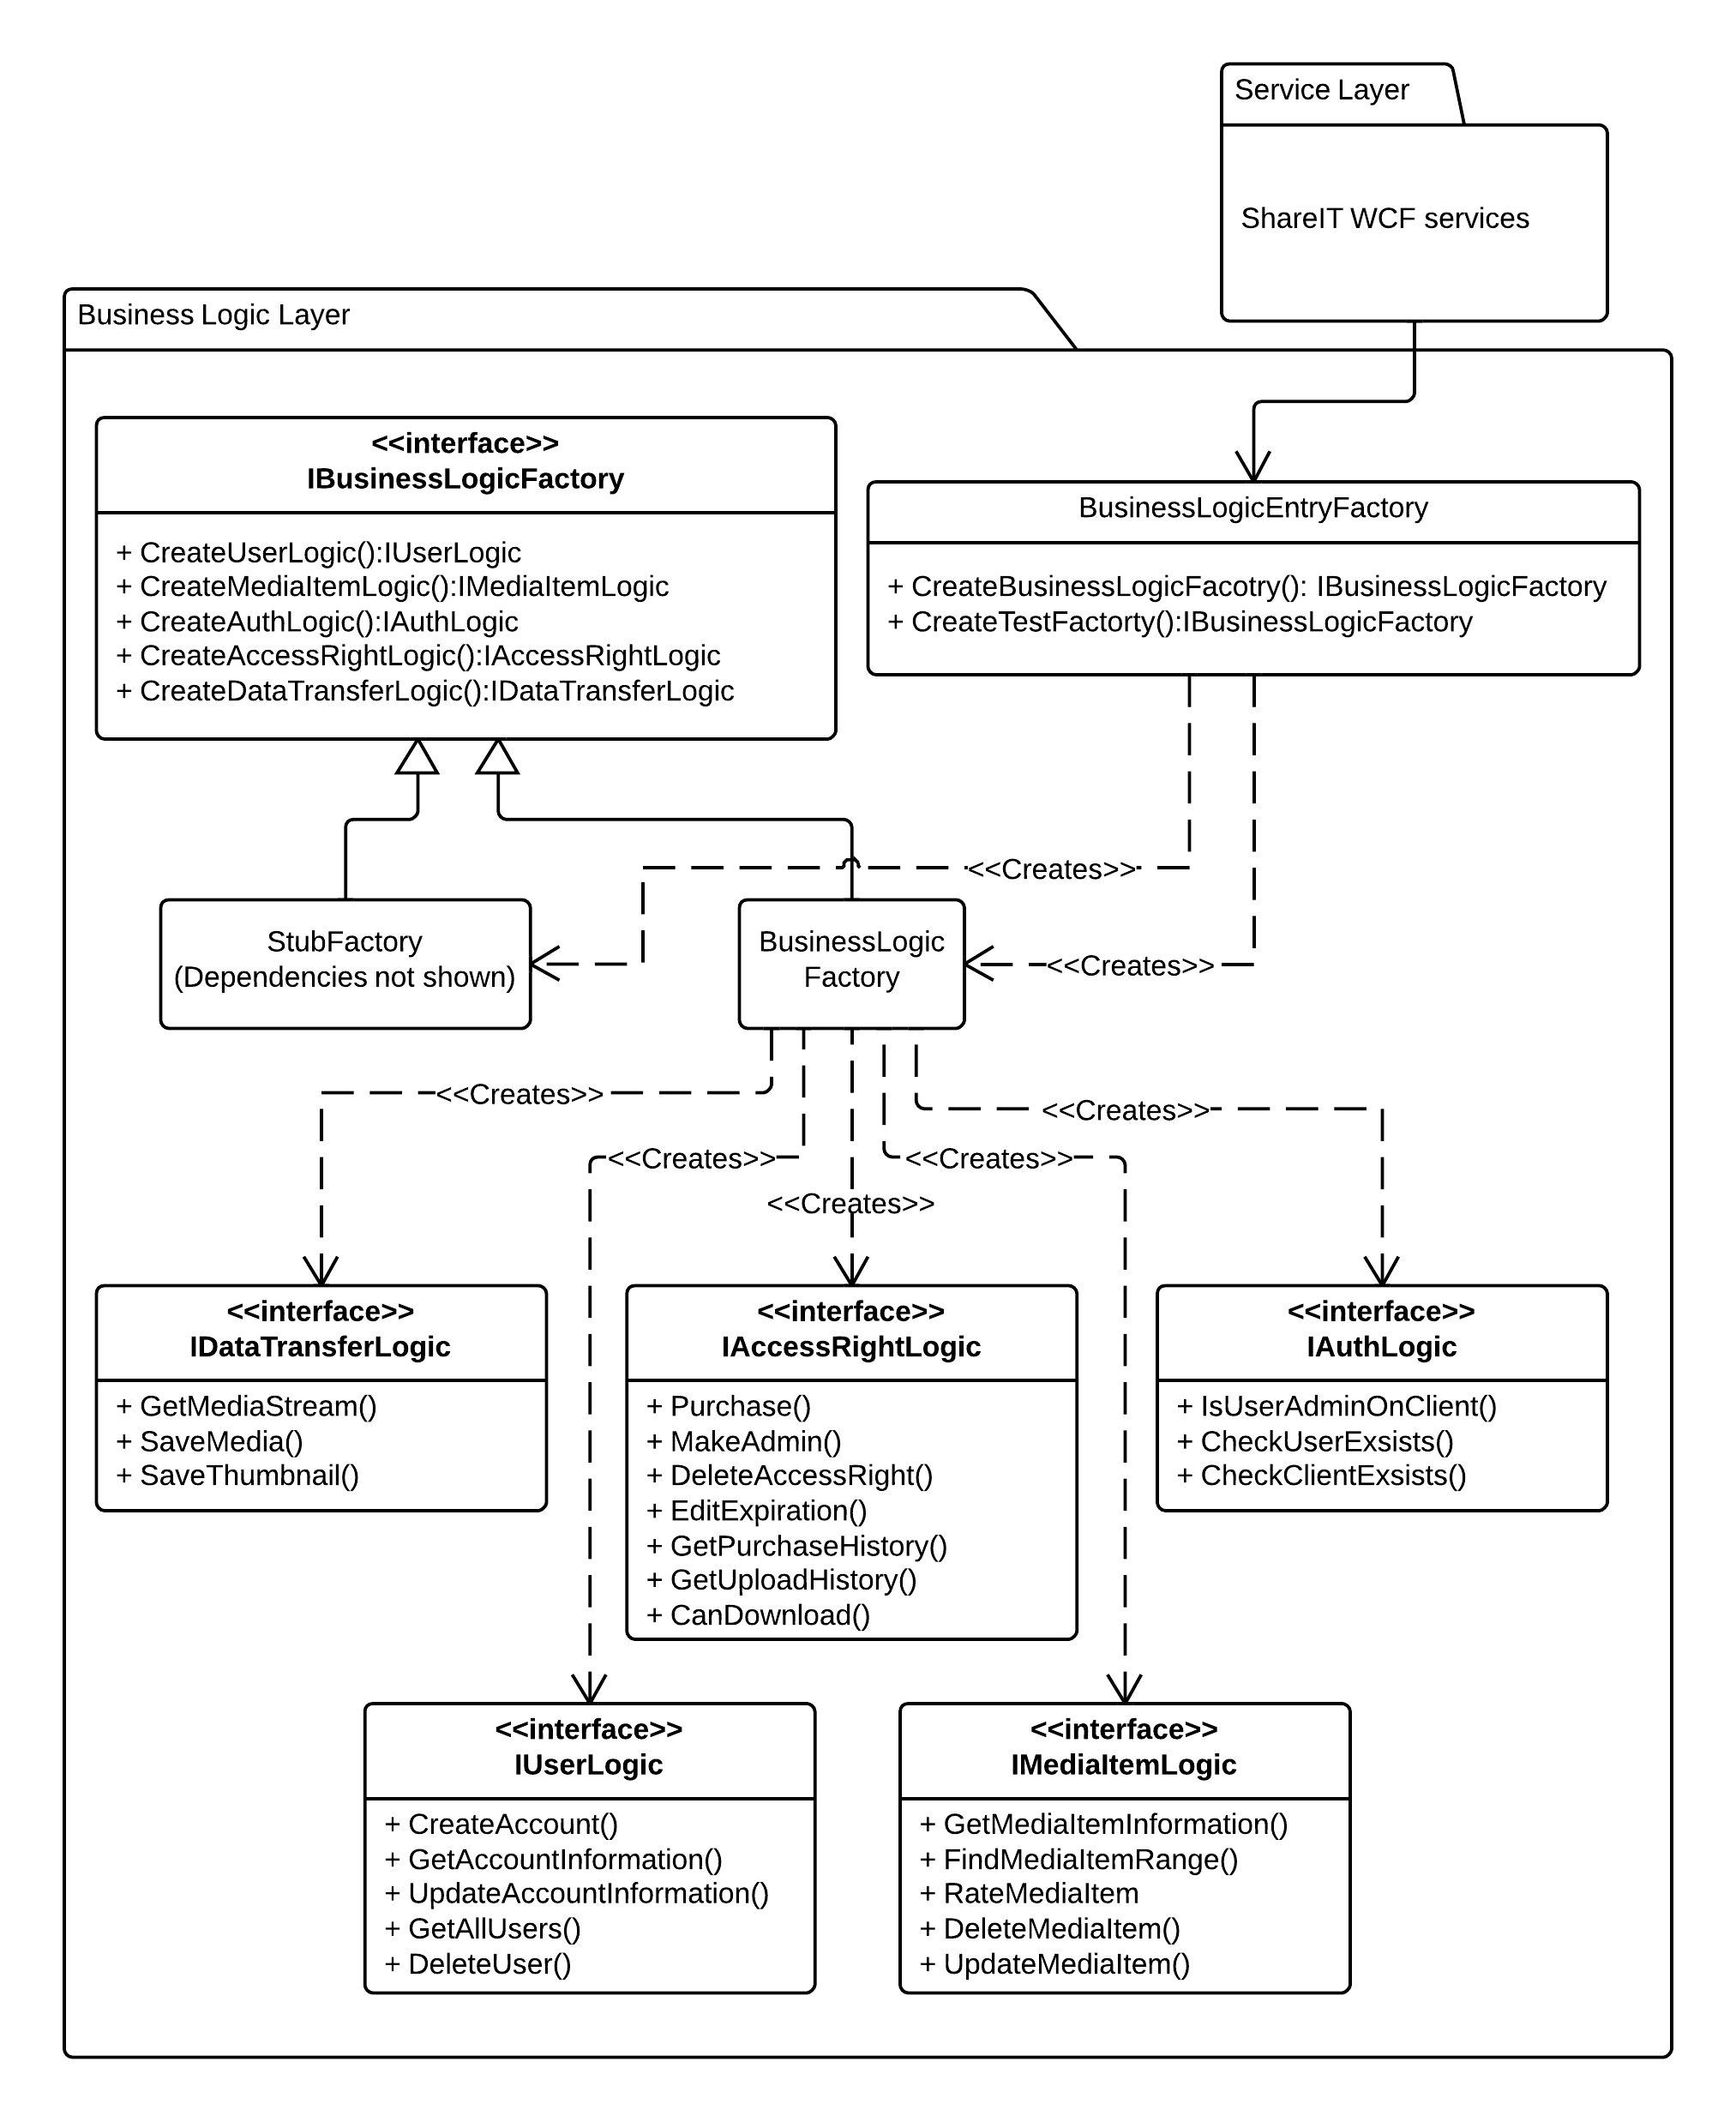
\includegraphics[width=\linewidth]{BLLclassdiagram.png}
\caption{Business Logic Layer class diagram (Not all classes are shown)}
\label{fig:BLLclassdiagram}
\end{figure}

%\begin{landscape}
%
%\newgeometry{left=1.5cm,right=-3cm}
%
%\subsection{Class Diagrams}
%
%\begin{figure}[!h]
%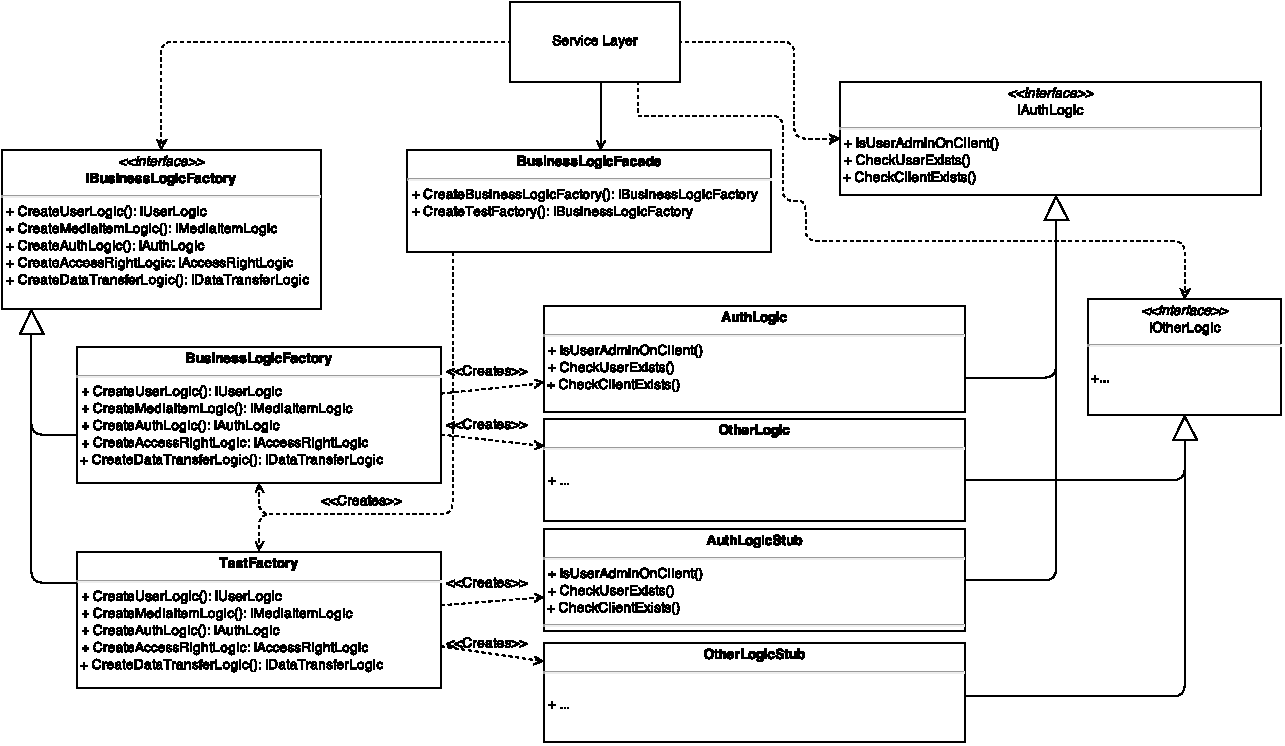
\includegraphics[ scale=1.2]{BusinessLogicLayerDiagram1.pdf}
%\caption{Class diagram showing the use of the Abstract Factory pattern}
%\label{fig:BusinessLogic_AbstractFactory}
%\end{figure}
%
%\end{landscape}


\newgeometry{left=5.5cm,bottom=1.5cm}

\begin{landscape}

\begin{figure}[!h]
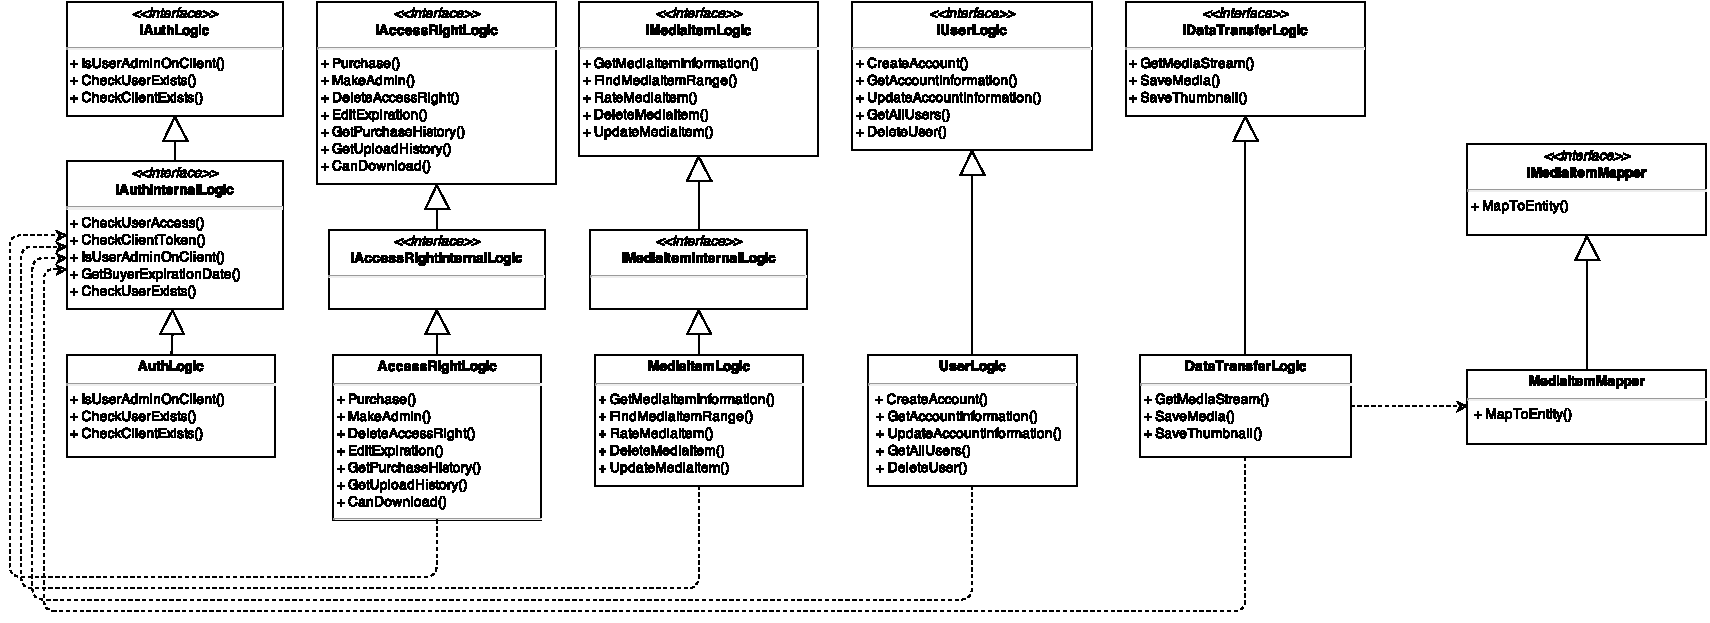
\includegraphics[ scale=0.9]{BusinessLogicLayerDiagram2.pdf}
\caption{Class diagram showing internal interfaces}
\label{fig:BusinessLogic_InternalInterfaces}
\end{figure}

\end{landscape}

\restoregeometry


% <-- HEAD


% ------
%Figure \ref{fig:BusinessLogic_AbstractFactory} above shows the class structure in the Business Logic Layer. The Entry Factory consists of a single concrete class which in our case is the BusinessLogicEntryFactory class. The BusinessLogicEntryFactory class makes it possible to get hold of the concrete factories without exposing the factories to the Service Layer.

%Underneath the Entry Factory lies the Abstract Factory pattern which starts with the Abstract Factory interface which in our case is the IBusinessLogicFactory. This interface specifies a method for creating each of the Abstract Products in this Abstract Factory. The Abstract Products are IAuthLogic, IUserLogic, IMediaItemLogic, IAccessRightLogic and IDataTransferLogic. We then have two concrete implementations of this interface and those are the BusinessLogicFactory and the TestFactory classes. Each of the concrete factories can then produce an instance of a concrete implementation of each Abstract Product. These concrete implementations must implement the Abstract Product interface which contains the methods that are exposed to the Service Layer. But they must also implement an internal interface (ie. IAuthInternalLogic) which specifies methods that are used internally in the Business Logic Layer as shown in figure \ref{fig:BusinessLogic_InternalInterfaces} above. These internal interfaces make it possible for the different concrete logic classes to expose methods to one another but not to the Service Layer. In our implementation all the logic classes use the authentication methods specified in the IAuthInternalLogic interface to authenticate users, admins and clients.
% --->


\end{document}